\documentclass[aspectratio=169,11pt]{beamer}

\usepackage{fontspec}
\usepackage{polyglossia}
\setdefaultlanguage{russian}
\setotherlanguage{english}
\setsansfont{DejaVu Sans}
\setmainfont{DejaVu Serif}
\setmonofont{DejaVu Sans Mono}

\usepackage{amsmath,amssymb}
\usepackage{graphicx}
\usepackage{xcolor}

\usetheme{Madrid}
\usecolortheme{default}

\definecolor{darkblue}{RGB}{28,62,115}
\definecolor{midblue}{RGB}{55,91,150}
\definecolor{lightblue}{RGB}{232,239,249}
\definecolor{darkgray}{RGB}{45,48,54}

\setbeamercolor{normal text}{fg=darkgray,bg=white}
\setbeamercolor{structure}{fg=darkblue}
\setbeamercolor{frametitle}{fg=white,bg=darkblue}
\setbeamercolor{frametitle right}{fg=white,bg=darkblue}
\setbeamercolor{title}{fg=white,bg=darkblue}
\setbeamercolor{titlelike}{fg=white,bg=darkblue}
\setbeamercolor{subtitle}{fg=white,bg=darkblue}
\setbeamercolor{palette primary}{fg=white,bg=darkblue}
\setbeamercolor{palette secondary}{fg=white,bg=midblue}
\setbeamercolor{palette tertiary}{fg=white,bg=darkblue}
\setbeamercolor{palette quaternary}{fg=white,bg=darkblue}
\setbeamercolor{headline}{fg=white,bg=darkblue}
\setbeamercolor{section in head/foot}{fg=white,bg=darkblue}
\setbeamercolor{subsection in head/foot}{fg=white,bg=midblue}
\setbeamercolor{author in head/foot}{fg=white,bg=midblue}
\setbeamercolor{title in head/foot}{fg=white,bg=darkblue}
\setbeamercolor{date in head/foot}{fg=white,bg=midblue}
\setbeamercolor{block title}{fg=white,bg=darkblue}
\setbeamercolor{block title alerted}{fg=white,bg=darkblue}
\setbeamercolor{block title example}{fg=white,bg=darkblue}
\setbeamercolor{block body}{fg=darkgray,bg=lightblue}
\setbeamercolor{alerted text}{fg=darkblue}
\setbeamertemplate{navigation symbols}{}
\setbeamertemplate{footline}{}
\setbeamertemplate{caption}[numbered]
\setbeamertemplate{itemize item}{\color{darkblue}$\blacktriangleright$}
\graphicspath{{../графики/}}

\newcommand{\fitA}{5.382}
\newcommand{\fitB}{1.585}
\newcommand{\fitRMSE}{1.30\cdot10^{-3}}
\newcommand{\fitMAE}{7.75\cdot10^{-4}}
\newcommand{\fitN}{93}
\newcommand{\vdwTc}{1.006}
\newcommand{\vdwRhoc}{0.210}
\newcommand{\vdwPc}{0.0793}

\title[MD LJ-флюида и Ван-дер-Ваальс]{флюид Ленарда-Джонса:\\MD-изотермы и эффективная аппроксимация Ван-дер-Ваальса}
\author{Станислав Смекалин}
\institute{МФТИ, Б02-507}
\date{\today}

\begin{document}

\begin{frame}
    \titlepage
\end{frame}

\begin{frame}{Задача}
    \begin{columns}[T]
        \begin{column}{0.48\textwidth}
            \textbf{Модель MD}
            \[
            u(r)=4\varepsilon\left[\left(\frac{\sigma}{r}\right)^{12}
            -\left(\frac{\sigma}{r}\right)^6\right]
            \]
            \begin{itemize}
                \item $\sigma=\varepsilon=m=k_B=1$
                \item $NVT$, периодическая ячейка
                \item давление из вириала
            \end{itemize}
        \end{column}
        \begin{column}{0.48\textwidth}
            \textbf{Эффективная модель}
            \[
            P_{\mathrm{VdW}}=\frac{\rho T}{1-b\rho}-a\rho^2
            \]
            \begin{itemize}
                \item fit только в газовой области
                \item $a$ и $b$ не универсальны
                \item проверяется экстраполяция
            \end{itemize}
        \end{column}
    \end{columns}
\end{frame}

\begin{frame}{Расчёт}
    \begin{itemize}
        \item OpenMM, $N=2048$, $r_c=2.5$, $\Delta t=0.002$, Langevin $\gamma=1.0$.
        \item До пяти независимых seed для каждой точки.
        \item $0.7\leq T\leq1.5$, $0.0025\leq\rho\leq0.85$.
        \item Релаксация $2\cdot10^4$ шагов; измерение $2\cdot10^4$ или $5\cdot10^4$ шагов.
        \item Погрешность давления: разброс независимых средних по seed.
    \end{itemize}
\end{frame}

\begin{frame}{Изотермы}
    \begin{columns}[T]
        \begin{column}{0.67\textwidth}
            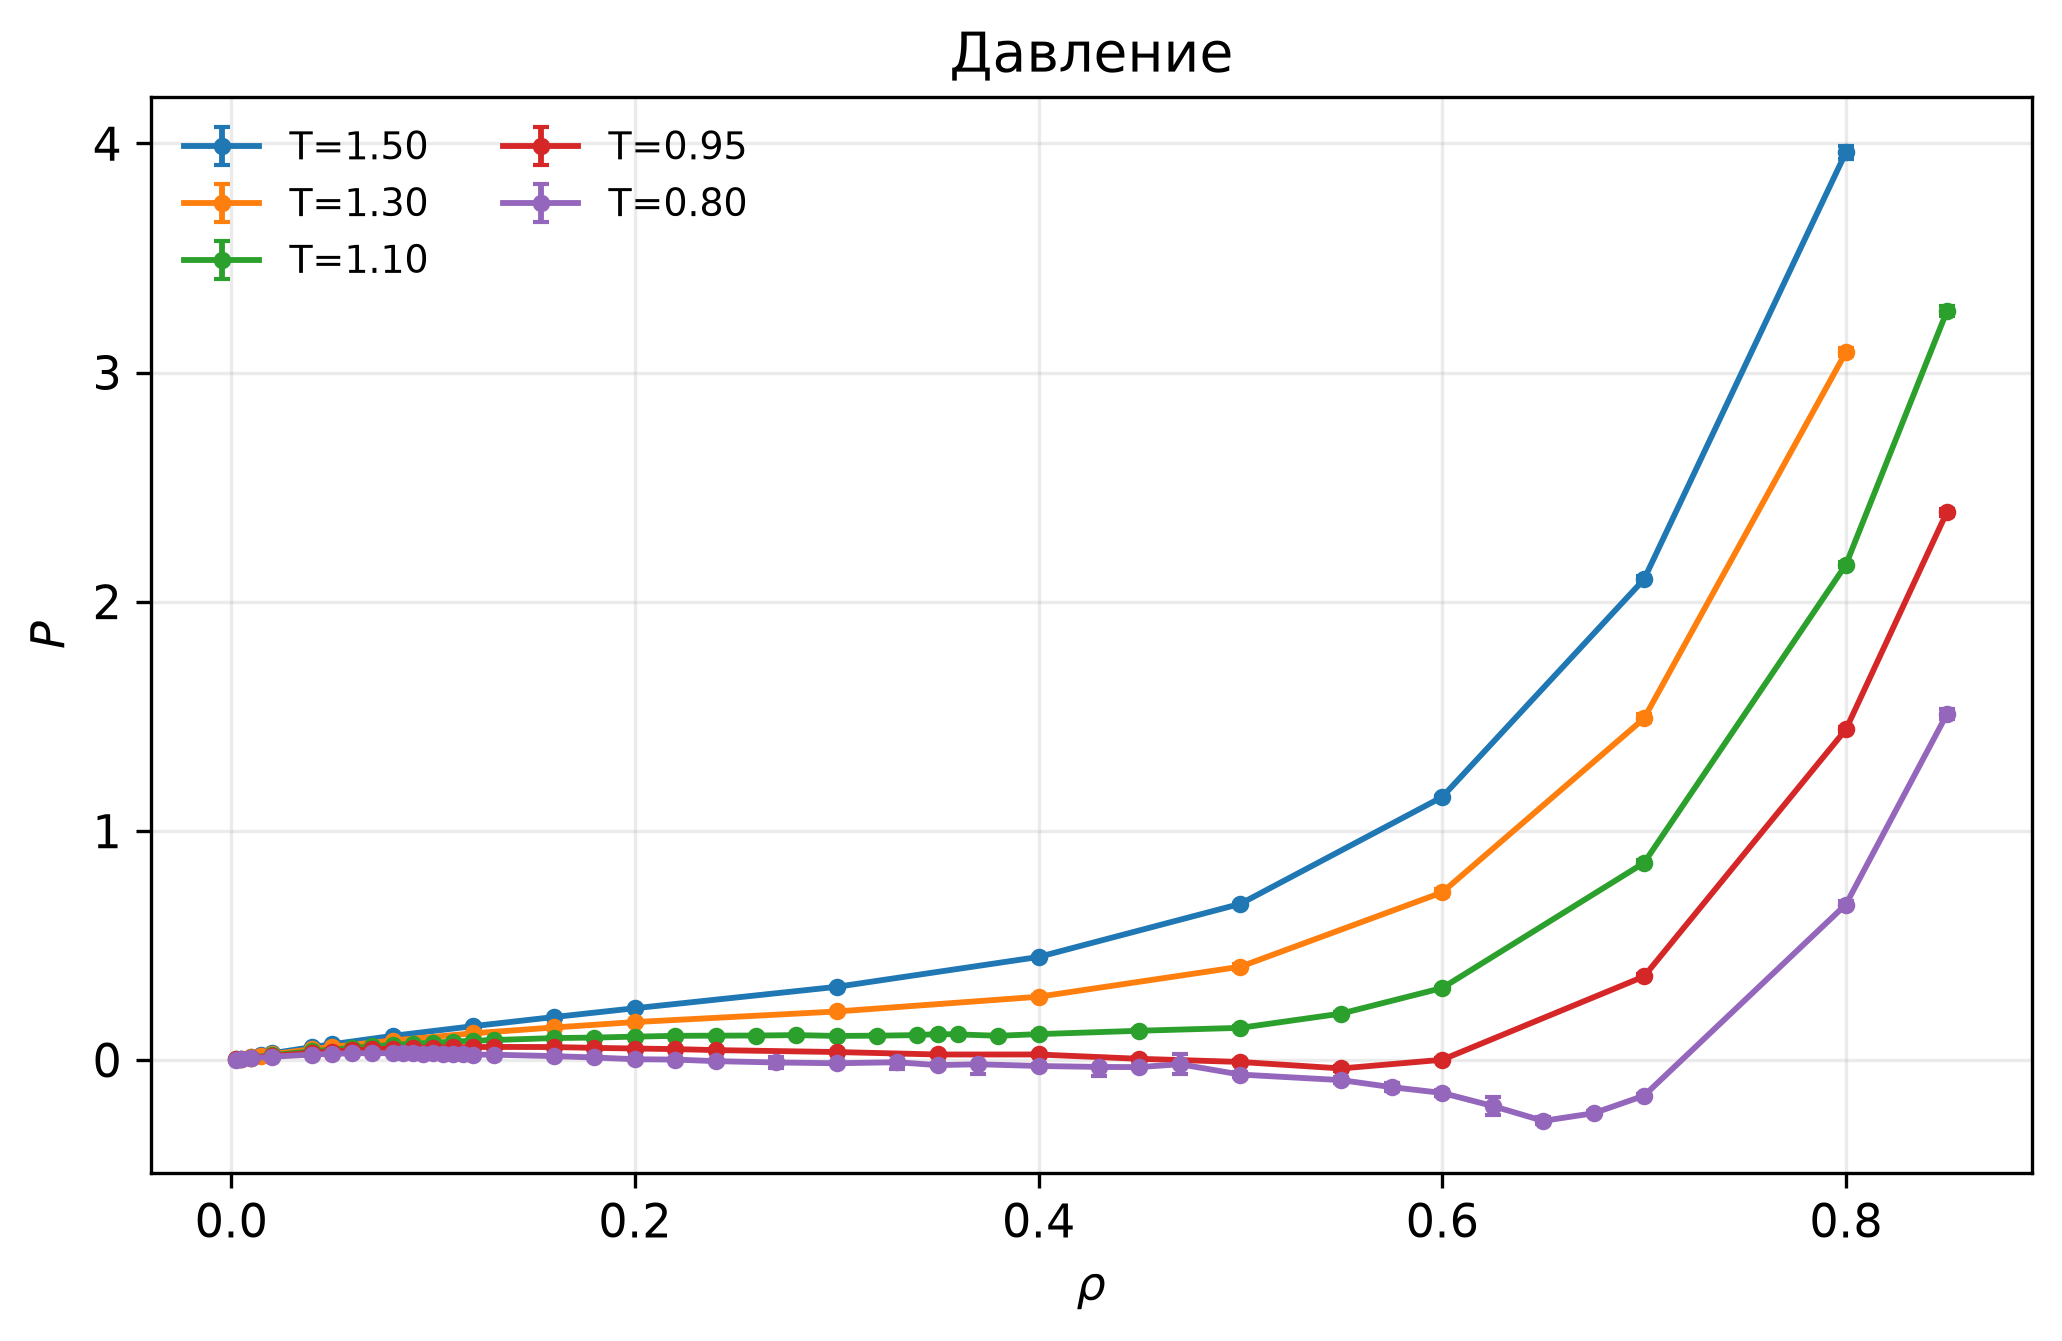
\includegraphics[width=\linewidth]{давление_от_плотности.png}
        \end{column}
        \begin{column}{0.30\textwidth}
            \begin{itemize}
                \item При малых $\rho$: $P\to\rho T$.
                \item Немонотонность видна до $T=1.0$.
                \item Оценка: $T_c\approx1.0$.
                \item При больших $\rho$ давление быстро растёт.
            \end{itemize}
        \end{column}
    \end{columns}
\end{frame}

\begin{frame}{Плотности до $\rho=0.3$}
    \begin{columns}[T]
        \begin{column}{0.68\textwidth}
            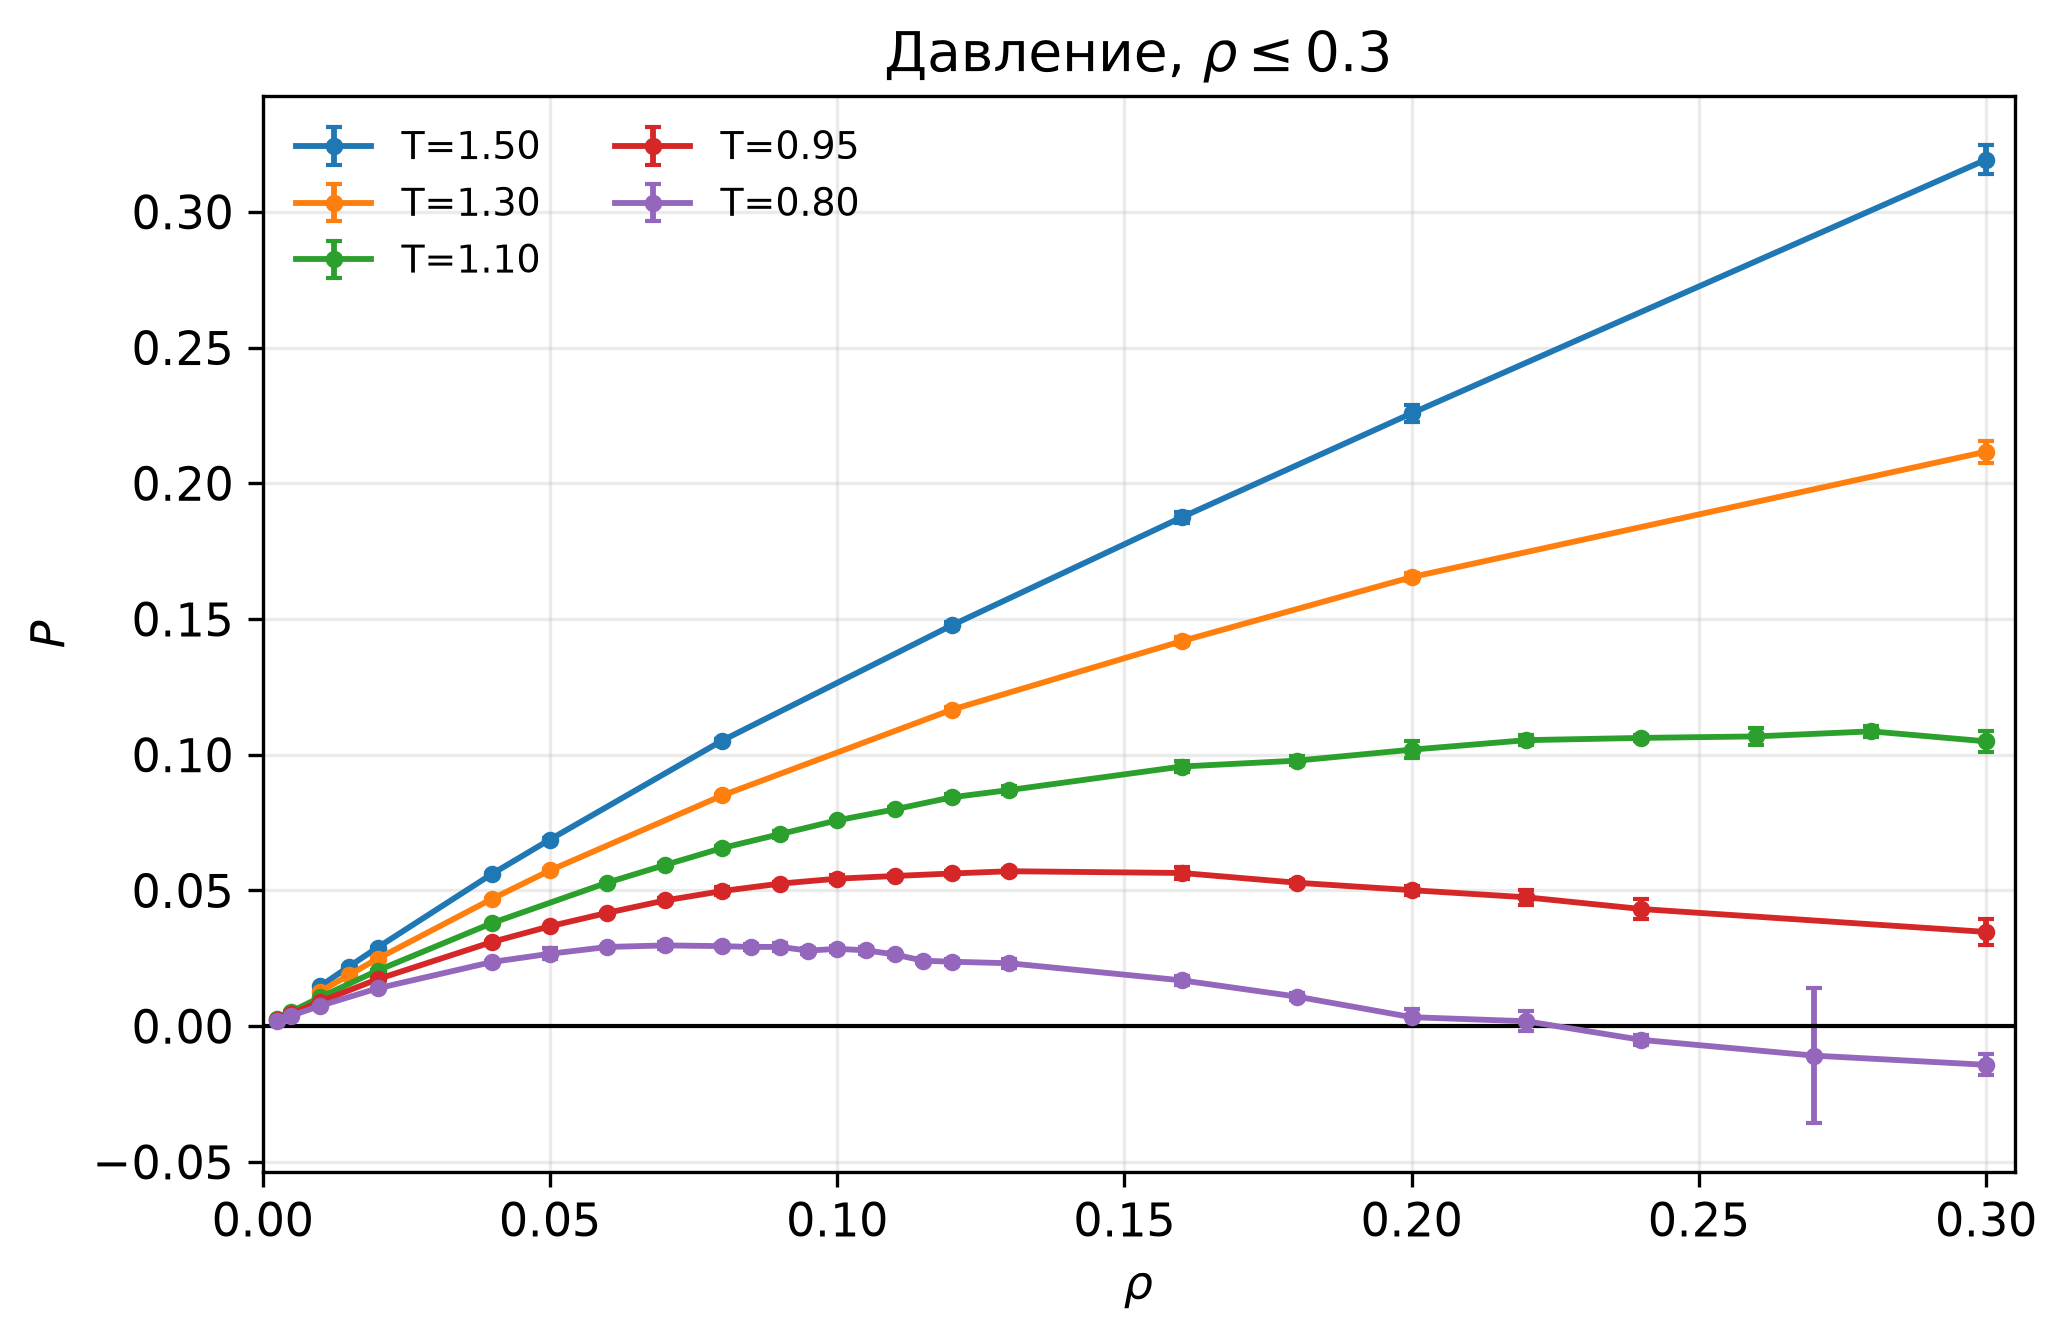
\includegraphics[width=\linewidth]{давление_малые_плотности.png}
        \end{column}
        \begin{column}{0.29\textwidth}
            \begin{itemize}
                \item Газовая ветвь хорошо разрешена.
                \item Fit выполняется при $T\geq1.1$, $\rho\leq0.20$.
                \item Ниже $T_c$ начинается заметная систематика отклонений.
            \end{itemize}
        \end{column}
    \end{columns}
\end{frame}

\begin{frame}{Подгонка Ван-дер-Ваальса}
    \begin{columns}[T]
        \begin{column}{0.50\textwidth}
            \begin{block}{Газовая область}
                \[
                T\geq1.1,\qquad \rho\leq0.20
                \]
                \[
                a=\fitA,\qquad b=\fitB
                \]
                \[
                \mathrm{RMSE}=\fitRMSE,\quad
                \mathrm{MAE}=\fitMAE
                \]
                \[
                N_{\mathrm{fit}}=\fitN
                \]
            \end{block}
        \end{column}
        \begin{column}{0.47\textwidth}
            \begin{block}{Критические параметры модели}
                \[
                T_c^{\mathrm{VdW}}=\vdwTc
                \]
                \[
                \rho_c^{\mathrm{VdW}}=\vdwRhoc,\qquad
                P_c^{\mathrm{VdW}}=\vdwPc
                \]
            \end{block}
            \vspace{0.5em}
            Температурный масштаб совпадает с MD-оценкой $T_c\approx1.0$.
        \end{column}
    \end{columns}
\end{frame}

\begin{frame}{Остатки}
    \begin{columns}[T]
        \begin{column}{0.68\textwidth}
            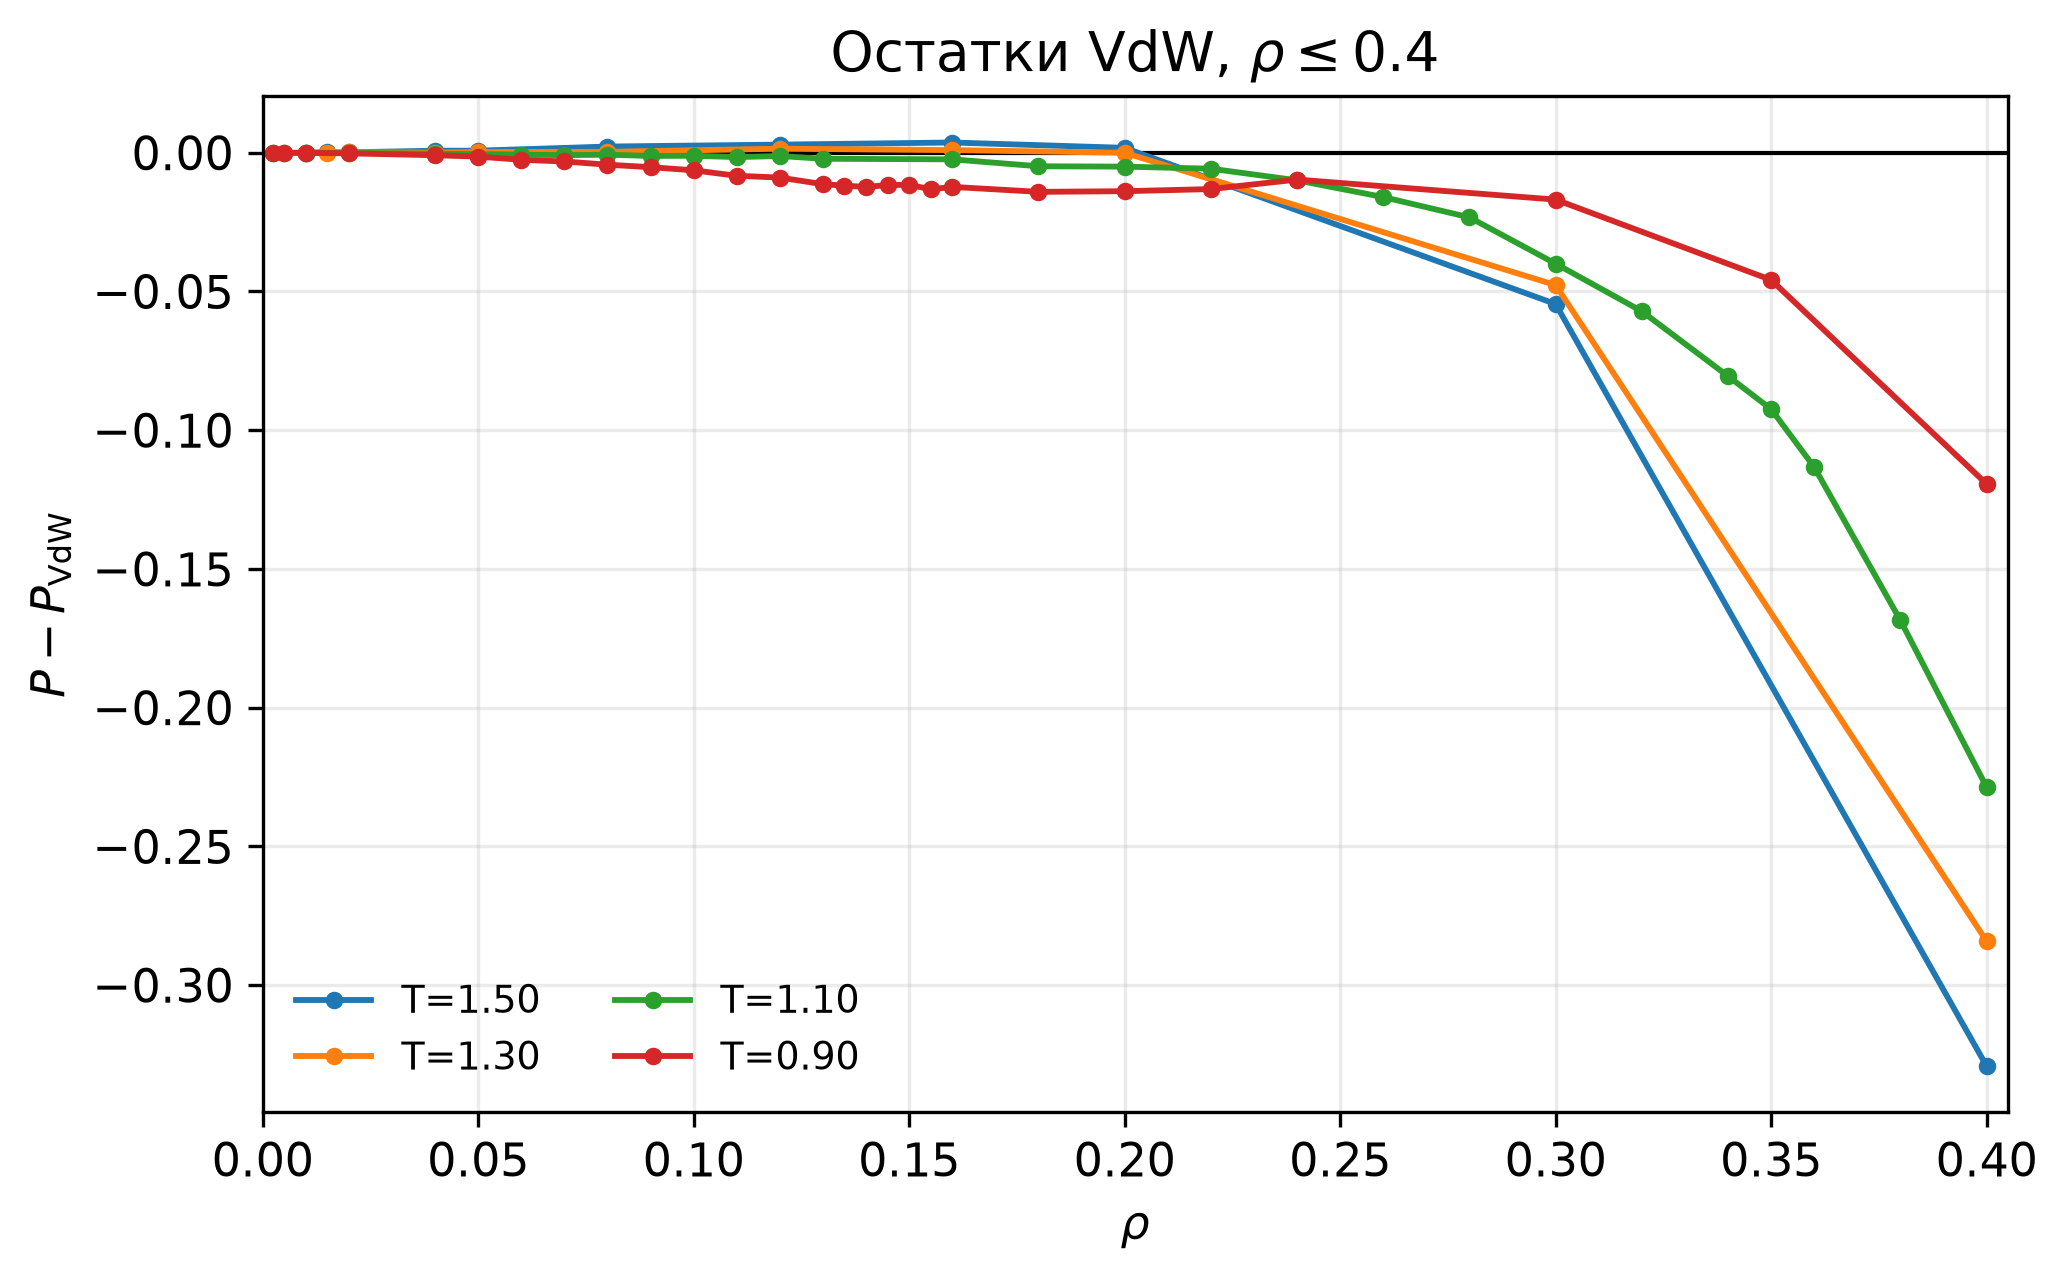
\includegraphics[width=\linewidth]{остатки_vdw_малые_плотности.png}
        \end{column}
        \begin{column}{0.29\textwidth}
            \begin{itemize}
                \item $\Delta P=P_{\mathrm{MD}}-P_{\mathrm{VdW}}$.
                \item Остатки имеют систематическую структуру.
                \item Ниже $T_c$ модель завышает давление.
                \item При $\rho>0.3$ количественная точность быстро теряется.
            \end{itemize}
        \end{column}
    \end{columns}
\end{frame}

\begin{frame}{Спинодаль и бинодаль}
    \begin{columns}[T]
        \begin{column}{0.68\textwidth}
            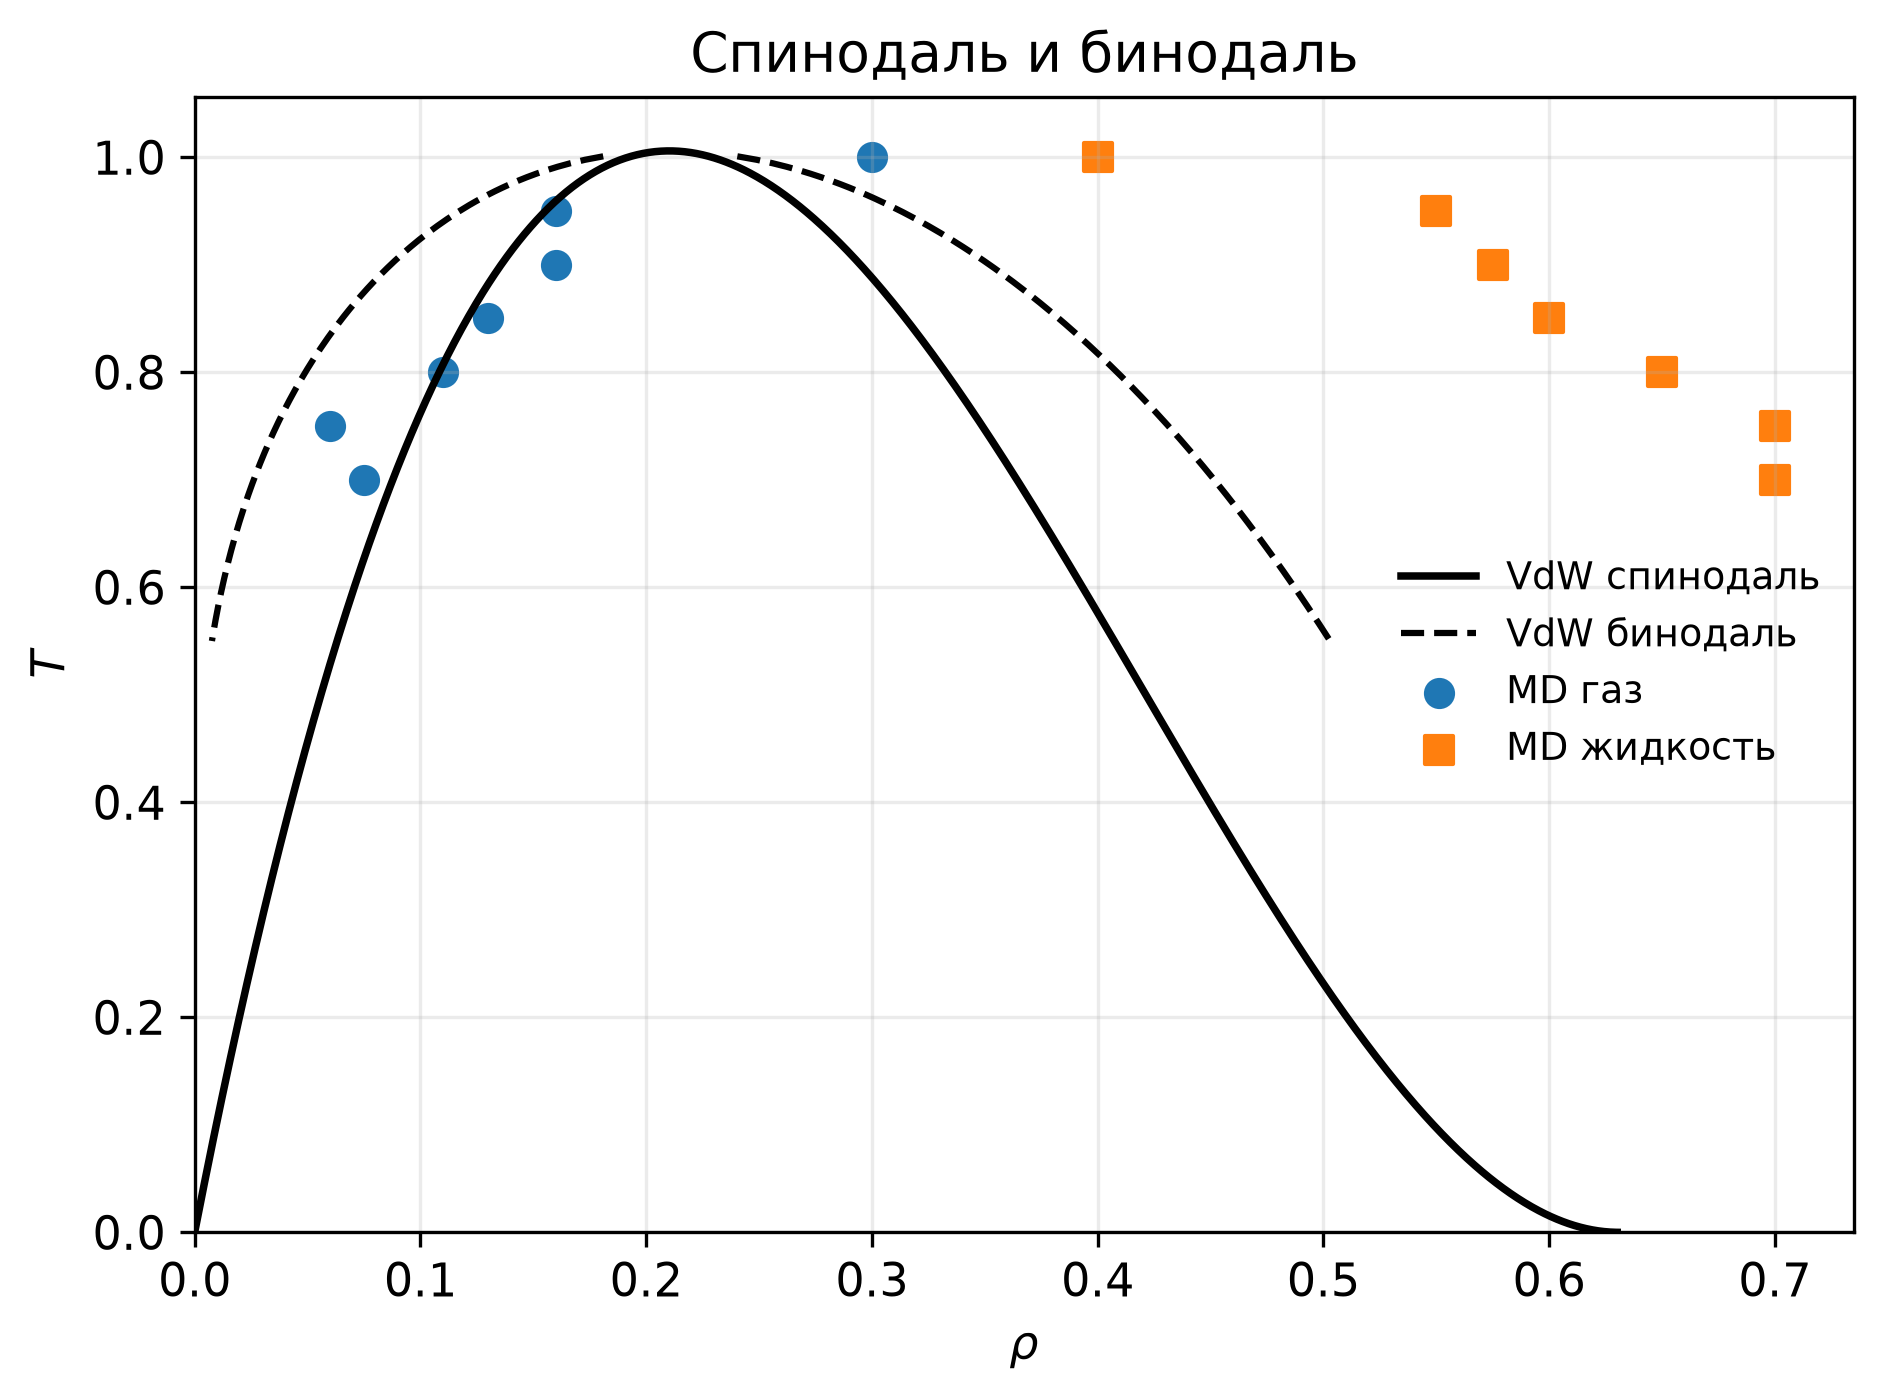
\includegraphics[width=\linewidth]{спинодаль_бинодаль_vdw.png}
        \end{column}
        \begin{column}{0.29\textwidth}
            \begin{itemize}
                \item Точки MD: границы немонотонных участков.
                \item Бинодаль MD не восстанавливалась.
                \item Газовая ветвь VdW согласуется хорошо.
                \item Жидкостная ветвь описана хуже.
            \end{itemize}
        \end{column}
    \end{columns}
\end{frame}

\begin{frame}{Потенциальная энергия}
    \begin{columns}[T]
        \begin{column}{0.68\textwidth}
            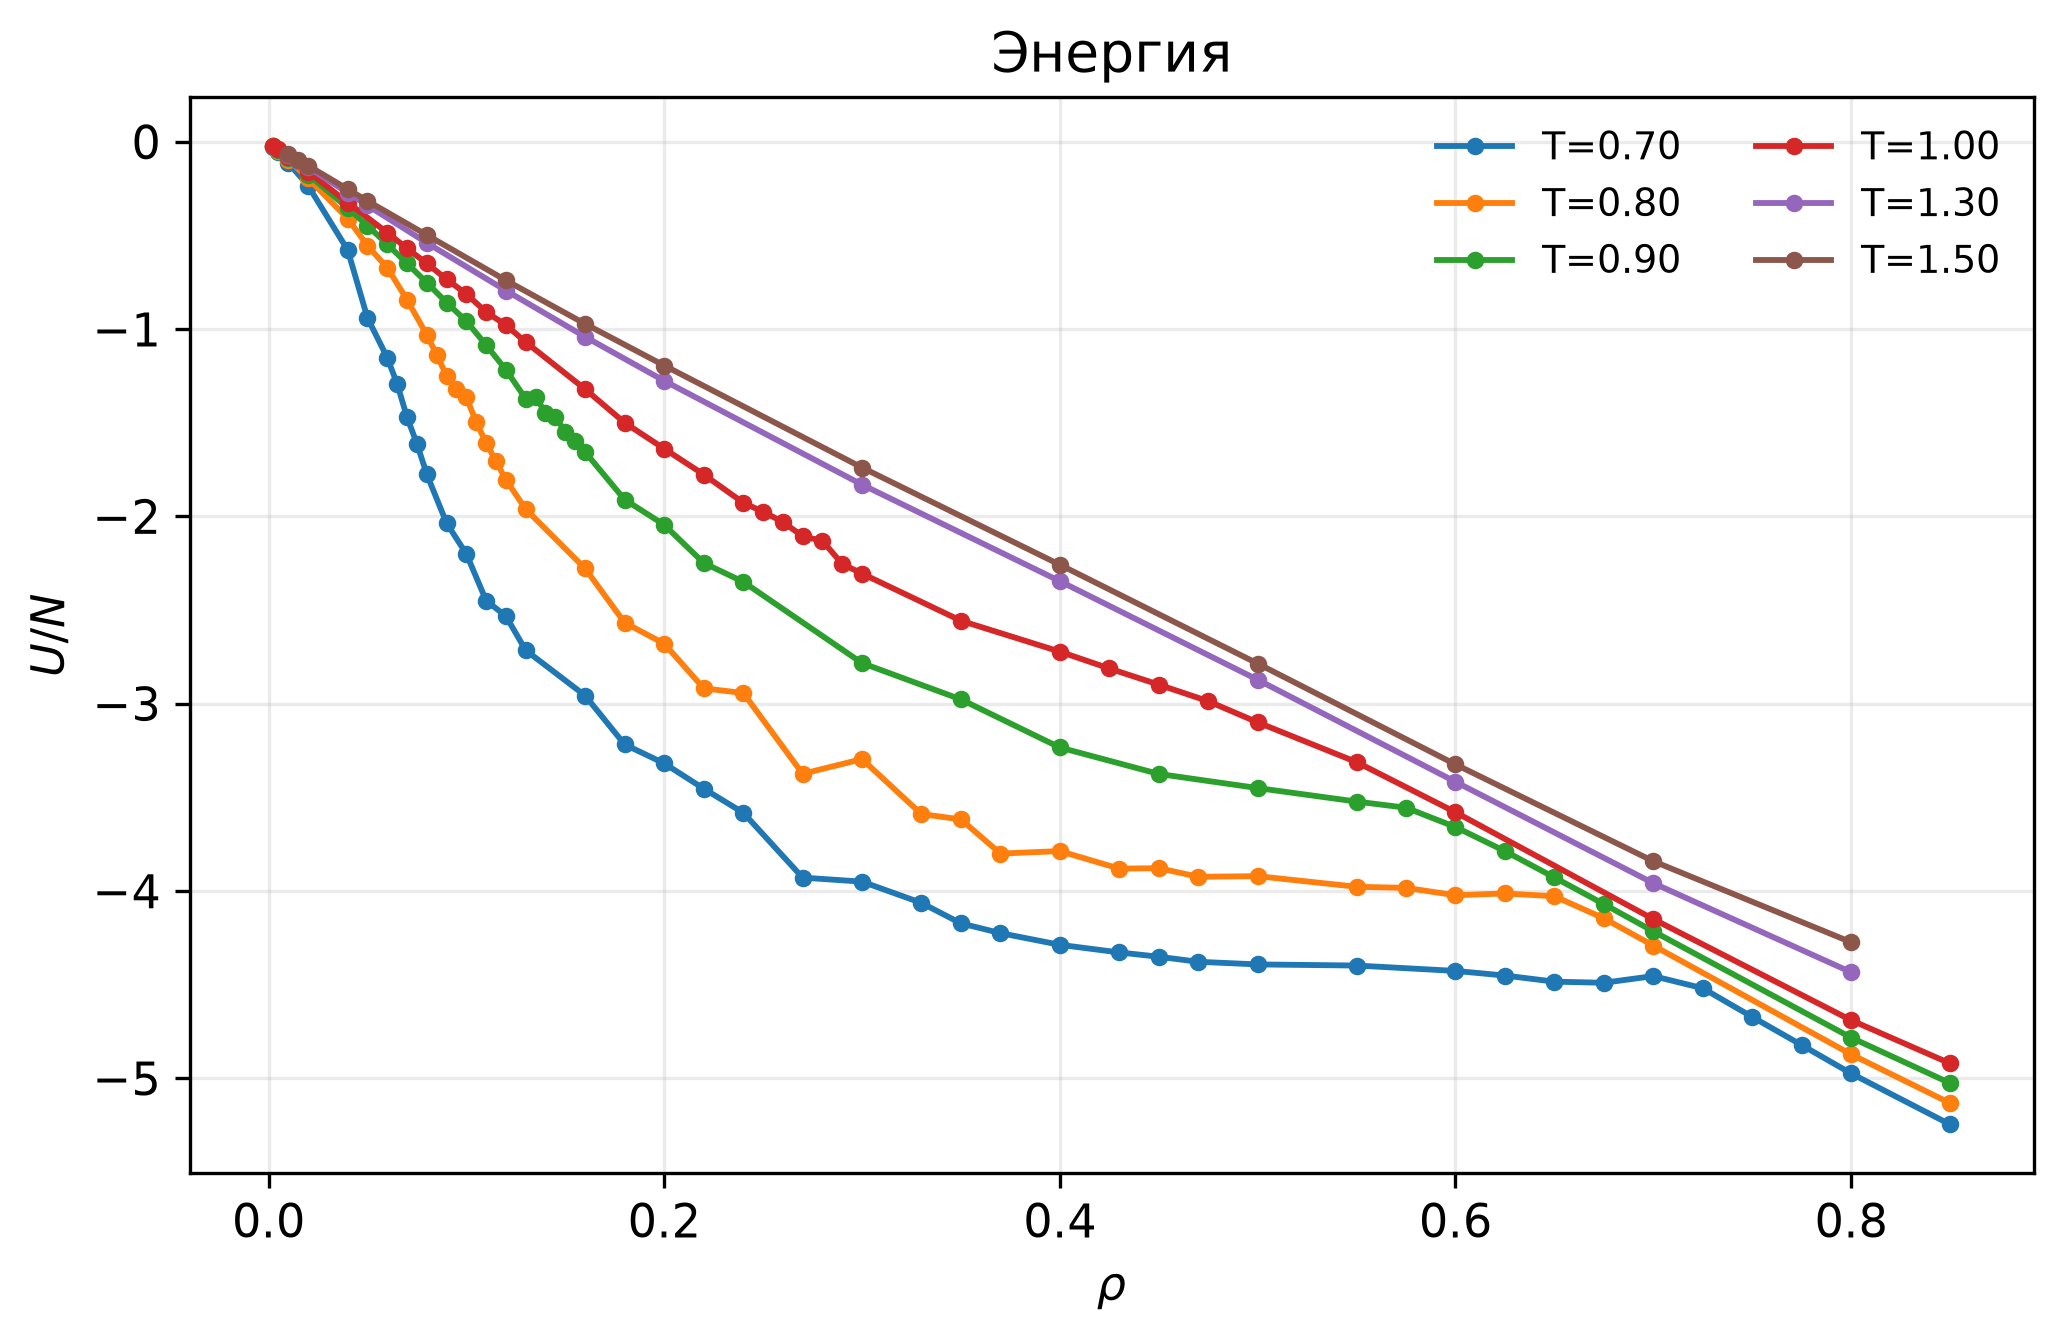
\includegraphics[width=\linewidth]{энергия_на_частицу.png}
        \end{column}
        \begin{column}{0.29\textwidth}
            \begin{itemize}
                \item При $T>1.1$ зависимость почти линейна.
                \item При меньших $T$ появляется прогиб.
                \item Это согласуется со структурной перестройкой.
            \end{itemize}
        \end{column}
    \end{columns}
\end{frame}

\begin{frame}{Неравновесное сжатие}
    \begin{block}{Назначение ролика}
        Качественная визуализация непрерывного изотермического сжатия LJ-флюида,
        а не равновесная изотерма.
    \end{block}
    \begin{itemize}
        \item $T=0.8$, $N=512$, $0.05\leq\rho\leq0.85$.
        \item Ячейка периодическая; термостат отводит тепло при сжатии.
        \item Траектория помогает увидеть уплотнение и структурную перестройку.
        \item Для количественных выводов используются только равновесные MD-точки.
    \end{itemize}
\end{frame}

\begin{frame}{Итоги}
    \begin{enumerate}
        \item MD воспроизводит переход от газа к области механической неустойчивости и плотному флюиду.
        \item Локальный fit Ван-дер-Ваальса хорошо описывает газовую область.
        \item Модель верно передаёт температурный масштаб и газовую ветвь спинодали.
        \item Жидкостная ветвь и область $\rho>0.3$ количественно описываются плохо.
        \item Поведение $U/N$ независимо подтверждает смену структурного режима.
    \end{enumerate}
\end{frame}

\appendix

\begin{frame}{Резерв: давление}
    \[
    P=\rho T+\frac{1}{3V}\left\langle
        \sum_{i<j}\mathbf r_{ij}\cdot\mathbf F_{ij}
    \right\rangle
    \]
    В периодической системе это изотропная часть среднего внутреннего напряжения.
\end{frame}

\begin{frame}{Резерв: спинодаль Ван-дер-Ваальса}
    \[
    \frac{\partial P}{\partial\rho}=\frac{T}{(1-b\rho)^2}-2a\rho
    \]
    \[
    T_{\mathrm{sp}}^{\mathrm{VdW}}(\rho)=2a\rho(1-b\rho)^2
    \]
\end{frame}

\end{document}
